	\section{Mission Planning Tool}
	To aid in development of a mission plan, a flight planning tool was developed to assess dwell time at various altitude and speeds.  The tool, \textit{mvss\_cameraFlightPlanning2}, allows the user to manually input flight parameter constants of altitude, flight speed, and image frame rate, as shown in \algref{alg:flightplan}.  
	
	\lstinputlisting[
	caption = {The flight planning tool is used to assist with calculating dwell time and spatial coverage for various flight parameters.},
	label = {alg:flightplan},
	style = Matlab-editor,
	basicstyle = \mlttfamily,
	firstline = 1,
	lastline = 7
	]{../../Matlab/mvss_cameraFlightPlanning2.m}
	
	The \textit{mvss\_cameraFlightPlanning2} algorithm automatically generates two plots, shown in \figref{fig:flightplots}.  The left plot is a spatial snapshot, showing what one image from each of the four cameras will cover spatially when it is centered at (0,0).  In the example shown, the images cover the entire 4km grid in the along-track distance.  The right plot shows the time dwell that each location would be imaged assuming a constant flight speed and altitude.  Higher, red values, represent a longer dwell time.  Each camera configuration yields a slightly different heat map of values, which can be useful for planning flight speeds and planning coverage.
		
	\begin{figure}[H]
		\centering
		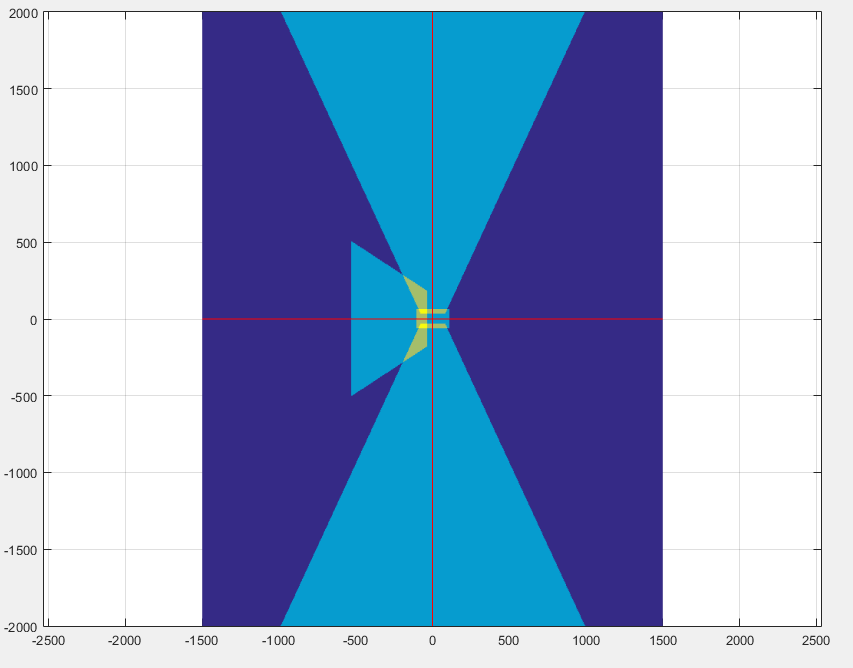
\includegraphics[scale = 0.3]{../figures/imageoverlap.png}
		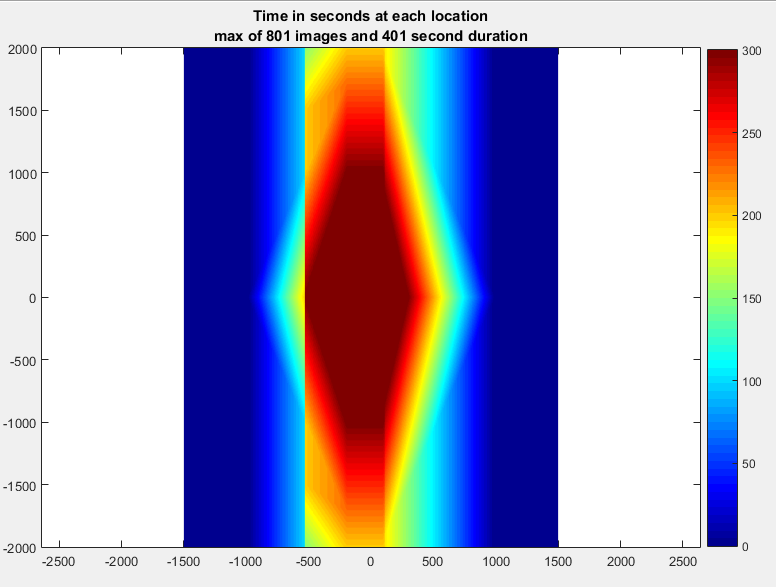
\includegraphics[scale = 0.341]{../figures/dwell.PNG}
		\caption{(Left) The spatial extent of one image snapshot is plotted with cross-track distance on the X-axis, and along-track distance on the Y-axis. (Right) The dwell time at every location in the cross-track(x-axis) and along-track(y-axis) is colored based on time in seconds, assuming a constant flight speed and altitude.}
		\label{fig:flightplots}
	\end{figure}
	\section{Flight Checklists}
	Three initial checklists are provided to ensure accurate and reliable data acquisitions.  The first checklist represents what should be done prior to a flight.  This includes checking all connections, batteries, SD cards, and settings to find any bugs before the actual acquisition.  The second checklist is to be used during the actual data collect.  This list should be improved to include more detailed X8 flight checklists, provided by 3DR robotics.  The final checklist describes how data should be stored and organized after a data collect.  This organization of data will make processing much more intuitive and user friendly. These checklists should be seen as an initial start, and should be iterated upon and improved based on user experience.
	\cleardoublepage
	\subsection{Pre Flight Checklist}
	\subsubsection*{Day Before Flight}
	\begin{easylist}[checklist]
		&& Charge GoPro Batteries
		&& Check Voltage/Charge PCB Batteries
		&& Clear SD Card for each camera
		&& Insert SD card for each camera
		&& Test Electronics to ensure it turns on and acquires PPS
		&& Clear SD card for electronics (DO NOT CLEAR CONFIG FILE)
		&& Make sure the config file still says 115200 Baud
		&& Place SD card for electronics into PCB slot
		&& Install Sensor on X8
		&& Charge Battery for X8
		&& Upload Mission to X8		
	\end{easylist}
	\subsubsection*{Once batteries are charged}
	\begin{easylist}[checklist]
			&& Install electronics tray
			&& Turn on electronics and ensure power light comes on and voltage is good
			&& Turn off electronics so power light goes off
			&& Ensure cameras turn on and are functional
			&& Ensure camera settings are set to 4K mode
			&& Place cameras in enclosures
			&&& Make sure each camera is in it's corresponding spot based on focal length
			&& Lock down each camera with screw
			&& Ensure cameras turn on and are functional after locking down
			&& Turn cameras all off so not to drain battery
			&& Place Cap on cameras to protect lenses
			&& Plug in the trigger cables, and handle cable management
			&& Plug in external GPS, and handle cable management
			&& lock down electronics tray with screw
	\end{easylist}
	
	\subsubsection*{One Hour before Flight}
	\begin{easylist}[checklist]
		&& Check Electronics	
		&&& Turn on electronics and ensure power light comes on and voltage is good
		&&& Turn off electronics so power light goes off
		&& Check Cameras
		&&& Ensure cameras turn on and are functional
		&&& Ensure camera settings are set to 4K mode
		&&& Ensure SD cards are in cameras
		&&& Power off all cameras
		&& Check X8
		&&& Check X8 Battery Voltage
	\end{easylist}
	\cleardoublepage
	\subsection{Flight Checklist}
	\begin{easylist}[checklist]
		&& Place X8 with sensor where you want to take off from
		&& Unscrew lens caps
		&& Power on Electronics. Do not power off until done with collect.
		&& Wait until White Light is Flashing, signifying PPS (may take a minute)
		&& Power on X8 and initialize
		&& Wait until X8 is initialized and ready to takeoff
		&& Turn on Each camera
		&& Ensure each is set to 4k mode
		&& Press record on each camera
		&& Set X8 flying
		&& Land X8
		&& Stop recording on each camera
		&&& Make note of any cameras are off
		&&& Make note of the PPS status 
		&& Turn off the Electronics via the panel switch
		&& Turn Off X8
		&& Place Lens Caps on sensor to protect lenses
	\end{easylist}
	
	\cleardoublepage
	\section{Post Flight Checklist}
	\begin{easylist}[checklist]
		&& Extract Data and organize, per \ref{sec:rawdata}
		&&& Different `data collect ID' should be saved for each collect on a day
		&&& Extract the logfileNNN.txt from PCB SD card
		&&& Extract Each Camera *.MP4 files
		&&& Extract SD card, from the X8FlightLog from the autopilot 
		&& Task someone with processing the Lidar or GPS surveys
		&& Charge GoPro Batteries
		&& Charge PCB battery
		&& Double check all data is backed up
		&& Triple check all data is backed up
		&& Clear SD cards
		&&& Clear Camera SD cards
		&&& Clear Log SD card (except config file)
		&&& Clear X8 SD card
		&& Place SD cards back in cameras, PCB, and X8
		&& Store equipment
	\end{easylist}
	\cleardoublepage
	\section{Data Management}
	\subsection{Raw Data Structure}\label{sec:rawdata}
	\dirtree{%
		.1 \treeDB{DataDepot}.
		.2 \treeFolder{MVSS2}.
		.3 \treeFolder{yyyymmdd\_$<$datacollectID$>$}.
		.4 \treeFolder{data}.
		.5 \treeFolder{control}.
		.6 \treeTxt{gcps.txt}.
		.6 \treeLAS{LidarControl.las}.
		.5 \treeFolder{video}.
		.6 \treeFolder{$<$ Camera Name $>$ (eg. Back, Down, Front, Left)}.
		.7 \treeGopro{*.mp4}.
		.5 \treeFolder{log}.
		.6 \treeTxt{yyyymmdd\_$<$id$>$\_X8flightLog.txt (log from autopilot)}.
		.6 \treeTxt{yyyymmdd\_$<$id$>$\_LogNNNN.txt (log from electronics sd card)}.
		.5 \treeTxt{meta.txt (metadata text file created for each flight)}.
	}
	\cleardoublepage
	\subsection{Processed Data Structure}
	\dirtree{%
		.1 \treeDB{DataDepot}.
		.2 \treeFolder{MVSS2}.
		.3 \treeFolder{yyyymmdd\_$<$datacollectID$>$}.
		.4 \treeFolder{data}.
		.5 \treeFolder{control}.
		.6 \treeTxt{gcps.txt}.
		.6 \treeLAS{LidarControl.las}.
		.5 \treeFolder{video}.
		.6 \treeFolder{$<$ Camera Name $>$ (eg. Back, Down, Front, Left)}.
		.7 \treeGopro{*.mp4}.
		.7 \treeTxt{$<$mp4name$>$\_gopro2gps.txt}.
		.5 \treeFolder{imagery}.
		.6 \treeFolder{$<$ Process Name $>$ (eg. dt0pt5s, dt2s)}.
		.7 \treeFolder{$<$ Camera Name $>$ (eg. Back, Down, Front, Left)}.
		.8 \treeImg{\%06.0f\_$<$mp4name$>$.jpg}.
		.8 \treeTxt{iminfo\_$<$mp4name$>$.txt}.
		.8 \treeTxt{iminfo\_$<$mp4name$>$\_pos.txt}.
		.5 \treeFolder{log}.
		.6 \treeTxt{yyyymmdd\_$<$id$>$\_X8flightLog.txt (log from autopilot)}.
		.6 \treeTxt{yyyymmdd\_$<$id$>$\_LogNNNN.txt (log from electronics sd card)}.
		.6 \treeTxt{yyyymmdd\_$<$id$>$\_LogNNNN\_gps.txt (log from electronics sd card)}.
		.5 \treeTxt{meta.txt (metadata text file created for each flight)}.
		.4 \treeFolder{products}.
		.5 \treeFolder{pointcloud}.
		.6 \treePhotoscanFolder{$<$PhotoScan Project Name $>$}.
		.6 \treeTxt{photoscanlog.txt (point photoscan to save all commands to a logfile here)}.
		.6 \treeFolder{LAS}.
		.7 \treeLAS{$<$Pointcloud Name$>$.las (eg. Dense10GCPS, Optimzed5GCPs)}.
		.7 \treeTxt{$<$Pointcloud Name$>$\_meta.txt}.
		.5 \treeFolder{orthos}.
		.6 \treeFolder{$<$ Processing Name $>$ (descriptive name to describe the orthos)}.
		.7 \treeImg{\%06.0f.jpg}.
		.7 \treeTxt{iminfo\_$<$mp4name$>$.txt}.
	}